\documentclass[crop,tikz,ifthenelse]{standalone}

\usetikzlibrary{calc}
\usepackage{tkz-euclide}
\usetkzobj{all}

\begin{document}
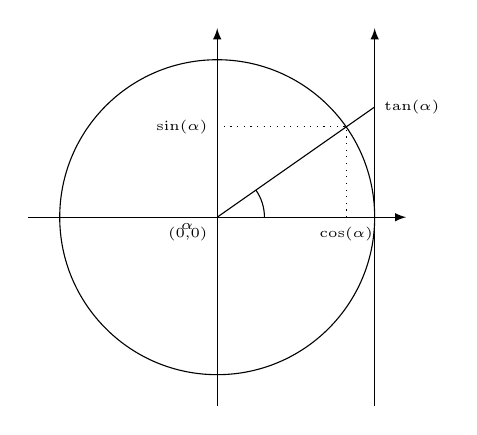
\begin{tikzpicture}[]

\coordinate(origin) at (0,0);
\coordinate(yaxis) at (0,6.5);
\coordinate(xaxis) at (6,0) ;

\draw (0,0) circle (2);
\draw[->,>= latex] (-2.4,0) -- (2.4,0);
\draw[->,>= latex] (0, -2.4) -- (0, 2.4);

// tangent line
\coordinate (tantop) at (2,2.4);
\coordinate (tanbottom) at (2,-2.4);
\draw[->,>= latex] (tanbottom) -- (tantop);

\coordinate (point) at (35:2);
\coordinate (origin) at (0,0);



\node[below left] {\tiny (0,0)};

\coordinate (procsin) at ($(origin)!(point)!(yaxis)$);
\coordinate (projcos) at ($(origin)!(point)!(xaxis)$) ;

\node[left]  at (procsin) {\tiny sin($\alpha$)};
\node[below] at (projcos) {\tiny cos($\alpha$)};

\draw[dotted] (projcos) -- (point) ;
\draw[dotted] (procsin) -- (point) ;



\coordinate (extended_point) at (2,1.4);%(35:3);
%\coordinate (tan_point) at (intersection of origin--extended_point and tanbottom -- tantop );

\node[right] at (extended_point) {\tiny tan($\alpha$)};

\tkzMarkAngle[fill= gray,size=0.6](xaxis,origin,extended_point);
\tkzLabelAngle[pos = 0.4](extended_point,origin,xaxis){\tiny $\alpha$};
\draw (origin) -- (extended_point) ;
\end{tikzpicture}
\end{document}